\documentclass[spanish,a4paper,11pt,twoside]{report}

%%%%%%%%%%%%%%%%%%%%%%%%%%%%%%%%%%%%%%%%%%%%%%%%%%%%%%%%%%%%%%%%%%%%%%%%%%%%%%%
\usepackage[dvips]{graphicx}
\usepackage[dvips]{epsfig}
\usepackage[latin1]{inputenc}
%\usepackage[utf8]{inputenc}
\usepackage[spanish]{babel}
\usepackage{alltt}
\usepackage{templates/algorithm}
\usepackage{templates/algorithmic}
\usepackage{templates/multirow}

%%%%%%%%%%%%%%%%%%%%%%%%%%%%%%%%%%%%%%%%%%%%%%%%%%%%%%%%%%%%%%%%%%%%%%%%%%%%%%%

\newcommand{\SONY}{{\sc Sony}}
\newcommand{\MICROSOFT}{{\sc Microsoft}}
\newcommand{\GCC}{\textsf{\textsc{G}CC}}
\newcommand{\INTEL}{\textsf{\textsc{I}ntel}}

%%% Traducimos el pseudocodigo
\renewcommand{\algorithmicwhile}{\textbf{mientras}}
\renewcommand{\algorithmicend}{\textbf{fin}}
\renewcommand{\algorithmicdo}{\textbf{hacer}}
\renewcommand{\algorithmicif}{\textbf{si}}
\renewcommand{\algorithmicthen}{\textbf{entonces}}
\renewcommand{\algorithmicrepeat}{\textbf{repetir}}
\renewcommand{\algorithmicuntil}{\textbf{hasta que}}
\renewcommand{\algorithmicelse}{\textbf{en otro caso}}
\renewcommand{\algorithmicfor}{\textbf{para}}

%\newcommand{\RETURN}{\textbf{retornar} }
\newcommand{\RET}{\STATE \textbf{retornar} }
\newcommand{\TO}{\textbf{hasta} }
\newcommand{\AND}{\textbf{y} }
\newcommand{\OR}{\textbf{o} }

%%%%%%%%%%%%%%%%% Creamos un entorno para listar c�digo fuente %%%%%%%%%%%%%%%
\newenvironment{sourcecode}
{\begin{list}{}{\setlength{\leftmargin}{1em}}\item\scriptsize\bfseries}
{\end{list}}

\newenvironment{littlesourcecode}
{\begin{list}{}{\setlength{\leftmargin}{1em}}\item\tiny\bfseries}
{\end{list}}

\newenvironment{summary}
{\par\noindent\begin{center}\textbf{Abstract}\end{center}\begin{itshape}\par\noindent}
{\end{itshape}}

\newenvironment{keywords}
{\begin{list}{}{\setlength{\leftmargin}{1em}}\item[\hskip\labelsep \bfseries Keywords:]}
{\end{list}}

\newenvironment{palabrasClave}
{\begin{list}{}{\setlength{\leftmargin}{1em}}\item[\hskip\labelsep \bfseries Palabras clave:]}
{\end{list}}


%%%%%%%%%%%%%%%%%%%%%%%%%%%%%%%%%%%%%%%%%%%%%%%%%%%%%%%%%%%%%%%%%%%%%%%%%%%%%%%
% Format
%%%%%%%%%%%%%%%%%%%%%%%%%%%%%%%%%%%%%%%%%%%%%%%%%%%%%%%%%%%%%%%%%%%%%%%%%%%%%%%

\oddsidemargin 5 mm
\evensidemargin 5 mm
\textwidth 15 cm
\input{amssym.def}
\voffset -3 cm

\pagestyle{empty}
\thispagestyle{empty}

\newcommand{\HRule}{\rule{\linewidth}{1mm}}
\setlength{\parindent}{0mm}
\setlength{\parskip}{0mm}
\vspace*{\stretch{1}}

%%%%%%%%%%%%%%%%%%%%%%%%%%%%%%%%%%%%%%%%%%%%%%%%%%%%%%%%%%%%%%%%%%%%%%%%%%%%%%%

\begin{document}

%%%%%%%%%%%%%%%%%%%%%%%%%%%%%%%%%%%%%%%%%%%%%%%%%%%%%%%%%%%%%%%%%%%%%%%%%%%%%%%
% First Page 
%%%%%%%%%%%%%%%%%%%%%%%%%%%%%%%%%%%%%%%%%%%%%%%%%%%%%%%%%%%%%%%%%%%%%%%%%%%%%%%


\begin{center}
\includegraphics[width=0.2\textwidth]{images/logotipo-secundario-ULL}\\[0.25cm]
\end{center}

\HRule

\begin{center}
        {\Huge Series de potencias Taylor. } \\[2.5mm] 
        {\Huge Funci�n Ln(x)} \\[2.5mm]
        {\Large Yoselin Armas Ramos y Bianca E. Kennedy Gim�nez} \\[5mm]
        {\Large \textit{GAII}} \\[5mm]


        {\em T�cnicas Experimentales. $1^{er}$ curso. $2^{do}$ semestre} \\[5mm]
        Facultad de Matem�ticas \\[5mm]
        
        Universidad de La Laguna \\
\end{center}
\HRule
\vspace*{\stretch{2}}
\begin{center}
  La Laguna, \today 
\end{center}
%\cleardoublepage
%%%%%%%%%%%%%%%%%%%%%%%%%%%%%%%%%%%%%%%%%%%%%%%%%%%%%%%%%%%%%%%%%%%%%%%%%%%%%%%

%%%%%%%%%%%%%%%%%%%%%%%%%%%%%%%%%%%%%%%%%%%%%%%%%%%%%%%%%%%%%%%%%%%%%%%%%%%%%%%
%\newpage{\pagestyle{empty}\cleardoublepage}

%\pagestyle{myheadings} %my head defined by markboth or markright
% No funciona bien \markboth sin "twoside" en \documentclass, pero al
% ponerlo se dan un mont�n de errores de underfull \vbox, con lo que no se
% ha puesto.
%\markboth{Yoselin Armas y Bianca Kennedy}{Series de Taylor}

%%%%%%%%%%%%%%%%%%%%%%%%%%%%%%%%%%%%%%%%%%%%%%%%%%%%%%%%%%%%%%%%%%%%%%%%%%%%%%%
%Numeracion en romanos
\renewcommand{\thepage}{\roman{page}}
\setcounter{page}{1}

%%%%%%%%%%%%%%%%%%%%%%%%%%%%%%%%%%%%%%%%%%%%%%%%%%%%%%%%%%%%%%%%%%%%%%%%%%%%%%%
  
\tableofcontents
\listoffigures
\cleardoublepage




%%%%%%%%%%%%%%%%%%%%%%%%%%%%%%%%%%%%%%%%%%%%%%%%%%%%%%%%%%%%%%%%%%%%%%%%%%%%%%%
%\newpage{\pagestyle{empty}\cleardoublepage}

%%%%%%%%%%%%%%%%%%%%%%%%%%%%%%%%%%%%%%%%%%%%%%%%%%%%%%%%%%%%%%%%%%%%%%%%%%%%%%%
%Numeracion a partir del capitulo I
\renewcommand{\thepage}{\arabic{page}}
\setcounter{page}{1}

\setlength{\parindent}{5mm}

%%%%%%%%%%%%%%%%%%%%%%%%%%%%%%%%%%%%%%%%%%%%%%%%%%%%%%%%%%%%%%%%%%%%%%%%%%%%%%%
\begin{abstract}

La asignatura de T�cnicas Experimentales nos ha aportado varios conocimientos sobre lo que era para nosotros un nuevo lenguaje de programaci�n.
Estos conocimientos adquiridos ser�n empleados en la investigaci�n de la Serie de Taylor aplicada a la funci�n $ln(x)$ . 
En el siguiente informe se puede observar el contenido del trabajo elaborado: historia, series de Taylor y Mclaurin, aplicaci�n matem�tica
y empleo de algoritmos para realizar varios experimentos que nos llevar�n a determinadas conclusiones.
\end{abstract}
%%%%%%%%%%%%%%%%%%%%%%%%%%%%%%%%%%%%%%%%%%%%%%%%%%%%%%%%%%%%%%%%%%%%%%%%%%%%%%%
\chapter{Motivaci�n y objetivos}
\label{chapter:obj}

%%%%%%%%%%%%%%%%%%%%%%%%%%%%%%%%%%%%%%%%%%%%%%%%%%%%%%%%%%%%%%%%%%%%%%%%%%%%%
% Chapter 1: Motivaci�n y Objetivos 
%%%%%%%%%%%%%%%%%%%%%%%%%%%%%%%%%%%%%%%%%%%%%%%%%%%%%%%%%%%%%%%%%%%%%%%%%%%%%%%

El objetivo de esta pr�ctica es demostrar los conocimientos adquiridos en Latex, Beamer y Python en el transcurso de la asignatura de T�cnicas Experimentales.
Aplicaremos los programas ya mencionados en la realizaci�n de un informe sobre la funci�n logaritmo neperiano y su desarrollo de Taylor.
Adem�s implementaremos un programa en Python que nos ayudar� a realizar varios experimentos para respaldar nuestras afirmaciones sobre el tema planteado.
%----------------------------------------------------------------------------------------------------
\section{Uso de Python,Beamer y Latex}
\label{1:sec:1}
\begin{itemize}
\item \LaTeX{} : Utilizaremos este programa en la realizaci�n del informe que presentaremos sobre $f(x)=Ln(x)$
\item Beamer : Recurriremos a la creaci�n de diapositivas para orientarnos en la exposici�n oral del trabajo.
\item Python : Crearemos un programa en lenguaje interpretado Python que utilizar� el desarrollo de Taylor para aproximar la funci�n Ln(x). 
As� como calcularemos el tiempo que tarda en realizar dicha aproximaci�n.
\end{itemize}
%---------------------------------------------------------------------------------






%%%%%%%%%%%%%%%%%%%%%%%%%%%%%%%%%%%%%%%%%%%%%%%%%%%%%%%%%%%%%%%%%%%%%%%%%%%%%%%
\chapter{Fundamentos te�ricos}
\label{chapter:teo}

\input{tex/cap2.tex}

%%%%%%%%%%%%%%%%%%%%%%%%%%%%%%%%%%%%%%%%%%%%%%%%%%%%%%%%%%%%%%%%%%%%%%%%%%%%%%%
\chapter{Procedimiento experimental}
\label{chapter:exp}

%%%%%%%%%%%%%%%%%%%%%%%%%%%%%%%%%%%%%%%%%%%%%%%%%%%%%%%%%%%%%%%%%%%%%%%%%%%%%%%
% Chapter 3: Procedimiento experimental 
%%%%%%%%%%%%%%%%%%%%%%%%%%%%%%%%%%%%%%%%%%%%%%%%%%%%%%%%%%%%%%%%%%%%%%%%%%%%%%%



%++++++++++++++++++++++++++++++++++++++++++++++++++++++++++++++++++++++++++++++
\section{Descripci�n de los experimentos}
\label{3:sec:1}
Tras elaborar un programa en Python capaz de calcular la aproximaci�n de la funci�n ln(x) mediante la serie de Taylor y el tiempo que tarda la m�quina en realizar esa aproximaci�n,
hemos realizado varios experimentos fijando el punto,el centro o el grado. Adem�s,tambi�n elaboramos un programa que nos calcula el error de dicha aproximaci�n.
Los experimentos realizados son los siguientes: 
\begin{enumerate}
\item Fijamos el grado de la Serie de Taylor(n=10),el punto en el que deseamos que se aplique (x=4) y variamos el centro.
\item Fijamos el grado de la Serie de Taylor (n=8), el centro (c=6) y variamos el punto en el que deseamos que se aplique.
\item Fijamos el centro(c=1) , el punto en el que deseamos que se aplique la aproximaci�n (x=2) y variamos el grado.
\end{enumerate}
%++++++++++++++++++++++++++++++++++++++++++++++++++++++++++++++++++++++++++++++
\section{Descripci�n del material}
\label{3:sec:2}
Todos los experimentos realizados se han llevado a cabo en un ordenador con las siguientes caracter�sticas:
\begin{verbatim}
 - Sistema operativo : Linux, Ubuntu.
 - Procesador: Intel(R) Core(TM) i3 
 - CPU :  M 350  @ 2.27GHz 
\end{verbatim}
\clearpage
%++++++++++++++++++++++++++++++++++++++++++++++++++++++++++++++++++++++++++++++
\section{Resultados obtenidos}
\subsection{Funci�n real del Logartimo Neperiano}
\begin{figure}[!th]

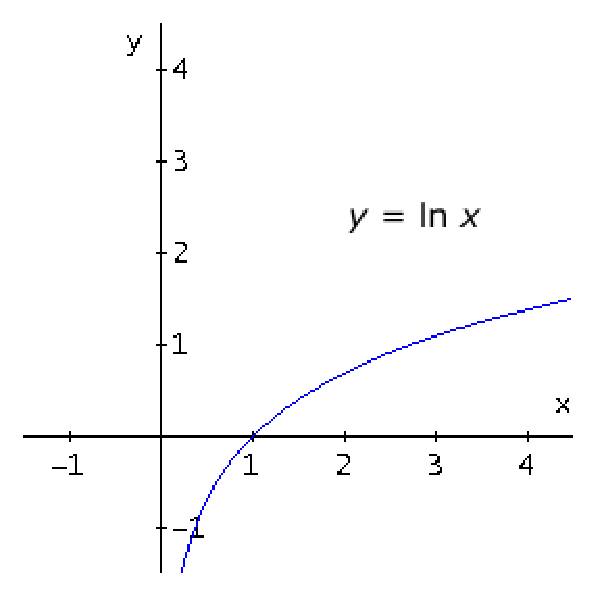
\includegraphics[width=0.30\textwidth]{images/fun053.eps}
\caption{Funci�n Logaritmo Neperiano}
\label{fig:1}

\end{figure}
\label{3:sec:3}

\subsection{Variaci�n del centro}
Fijando n=10 y x=4

\begin{tabular}{|l | r@{,}l |}
\hline
Si el valor de c= 2   & 1  & 33878210119487\\
\hline
Si el valor de c= 3   & 1  & 38629396788690\\
\hline 
Si el valor de c= 5   & 1  & 38629436340045\\
\hline
Si el valor de c= 30  & 1  & 48572417754861\\
\hline
Si el valor de c= 60  & 1  & 74292118557045\\
\hline
\end{tabular}


\subsection{Variaci�n del punto }
Fijando n=8 y c=6

\begin{tabular}{|l | r@{,}l |}
\hline
Si el valor de x= 8  &  2 & 07943719692636\\
\hline
Si el valor de x= 7  &  1 & 94591013946629\\
\hline
Si el valor de x= 6  &  1 & 79175946922805\\
\hline
Si el valor de x = 5 &  1 & 60943792540920\\
\hline
Si el valor de x= 4  & 1  & 38630243959407\\
\hline
\end{tabular}

\subsection{Variaci�n del grado }
Fijando x=2 y c=1

\begin{tabular}{|l | r@{,}l |}
\hline
Si el valor de n= 5     &  0 & 783333333333333\\
\hline
Si el valor de n= 15    &  0 & 725371850371850\\
\hline
Si el valor de n= 25    &  0 & 712747499542829\\
\hline
Si el valor de n= 200   &  0 & 690653430481824\\
\hline
Si el valor de n= 800   &  0 & 692522571184642\\
\hline
\end{tabular}

\clearpage
\subsection{Tiempo }
Tomamos los resultados de la tabla anterior y calculamos el tiempo que tarda el ordenador en obtener los resultados.

\begin{tabular}{|l | r@{,}l |}
\hline
Si el valor de n= 5     &  9 & 53674316406e-07\\
\hline
Si el valor de n= 15    &  9 & 53674316406e-07\\
\hline
Si el valor de n= 25    &  9 & 53674316406e-07\\
\hline
Si el valor de n= 200   &  1 & 19209289551e-06\\
\hline
Si el valor de n= 800   &  1 & 90734863281e-06\\
\hline

\end{tabular}
%------------------------------------------------------------------------------

%------------------------------------------------------------------------------

%++++++++++++++++++++++++++++++++++++++++++++++++++++++++++++++++++++++++++++++
\section{An�lisis de los resultados}
\label{3:sec:4}

\begin{itemize}
\item Variaci�n del centro: Variando el centro, fijando el grado (n=10) y el punto (x=4), podemos observar que cuanto m�s se aleja centro del punto menos acertado es el resultado.
\item Variaci�n del punto: Variando el punto, y fijando el centro (c=6) y el grado (n=8), observamos que si el punto es igual al centro el valor de la Serie de Taylor es  no conduce a ning�n error, ya que al ser iguales su diferencia es cero 
y nos da la imagen en ese punto o centro del logaritmo neperiano. Adem�s, vemos que si incrementamos la diferencia entre ambos puntos el resultado se aleja m�s del aut�ntico valor.
\item Variaci�n del grado: Al variar el grado y fijando el punto (x=2) y el centro (c=2), apreciamos que cuanto mayor es el grado m�s disminuye el error, por lo cual, si aunmentamos el valor del grado m�s precisos son los resultados. 
\item Tiempo: en cuanto al tiempo, el ordenador realiza los procesos m�s lento dependiendo del grado, ya que la ecuaci�n es m�s larga.
\end{itemize}


%%%%%%%%%%%%%%%%%%%%%%%%%%%%%%%%%%%%%%%%%%%%%%%%%%%%%%%%%%%%%%%%%%%%%%%%%%%%%%%
\chapter{Conclusiones}
\label{chapter:con}
%%%%%%%%%%%%%%%%%%%%%%%%%%%%%%%%%%%%%%%%%%%%%%%%%%%%%%%%%%%%%%%%%%%%%%%%%%%%%
% Chapter 4: Conclusiones y Trabajos Futuros 
%%%%%%%%%%%%%%%%%%%%%%%%%%%%%%%%%%%%%%%%%%%%%%%%%%%%%%%%%%%%%%%%%%%%%%%%%%%%%%%


%%%%%%%%%%%%%%%%%%%%%%%%%%%%%%%%%%%%%%%%%%%%%%%%%%%%%%%%%%%%%%%%%%%%%%%%%%%%%%%

%%%%%%%%%%%%%%%%%%%%%%%%%%%%%%%%%%%%%%%%%%%%%%%%%%%%%%%%%%%%%%%%%%%%%%%%%%%%%%%

\begin{appendix}

\chapter{Ap�ndice 1}
\title{Ap�ndice }
\label{appendix:1}

\section{Algoritmo XXX}
\label{Apendice1:XXX}

\begin{center}
\begin{footnotesize}
\begin{verbatim}
###################################################################################
# Fichero .py
###################################################################################
from sympy import *
import sys
 
def fac(grado):
  if grado == 0:
    return 1
  else:
    return grado * fac(grado-1)

def taylor(grado, punto, centro):
  c = Symbol('c')
  funcion = ln(c)
  suma = funcion.evalf(subs={c:centro})
  for i in range(1,grado+1):
    deriv = diff(funcion, c)
    termino = (deriv.evalf(subs={c:centro})/fac(i))*((punto-centro)**i)
    funcion = deriv
    suma += termino
  return suma

grado = int(raw_input('Introduzca el grado en el que desea que se aplique el desarrollo de Taylor: '))
punto = float(raw_input('Introduzca el punto en el que desea que se aplique el desarrollo de Taylor: '))
centro = float(raw_input('Introduzca el centro en el que desea que se aplique el desarrollo de Taylor: '))
suma = taylor(grado, punto, centro)
print 'El polinomio de Taylor es: ', suma

###################################################################################
\end{verbatim}
\end{footnotesize}
\end{center}



\end{appendix}

%%%%%%%%%%%%%%%%%%%%%%%%%%%%%%%%%%%%%%%%%%%%%%%%%%%%%%%%%%%%%%%%%%%%%%%%%%%%%%%
%%%%%%%%%%%%%%%%%%%%%%%%%%%%%%%%%%%%%%%%%%%%%%%%%%%%%%%%%%%%%%%%%%%%%%%%%%%%%%%
\addcontentsline{toc}{chapter}{Bibliograf�a}
\bibliographystyle{plain}


\bibliography{bib/references}
\nocite{*}

%%%%%%%%%%%%%%%%%%%%%%%%%%%%%%%%%%%%%%%%%%%%%%%%%%%%%%%%%%%%%%%%%%%%%%%%%%%%%%%

\end{document}